%\addcontentsline{toc}{chapter}{Development Process}
\chapter{Design}

%You should concentrate on the more important aspects of the design. It is essential that an overview is presented before going into detail. As well as describing the design adopted it must also explain what other designs were considered and why they were rejected.

%The design should describe what you expected to do, and might also explain areas that you had to revise after some investigation.

%Typically, for an object-oriented design, the discussion will focus on the choice of objects and classes and the allocation of methods to classes. The use made of reusable components should be described and their source referenced. Particularly important decisions concerning data structures usually affect the architecture of a system and so should be described here.

%How much material you include on detailed design and implementation will depend very much on the nature of the project. It should not be padded out. Think about the significant aspects of your system. For example, describe the design of the user interface if it is a critical aspect of your system, or provide detail about methods and data structures that are not trivial. Do not spend time on long lists of trivial items and repetitive descriptions. If in doubt about what is appropriate, speak to your supervisor.

%You should also identify any support tools that you used. You should discuss your choice of implementation tools - programming language, compilers, database management system, program development environment, etc.

%Some example sub-sections may be as follows, but the specific sections are for you to define.

As the application was developed in an iterative manner, over a series of sprints, class diagrams and design diagrams were not created at the very start of the project. Over a series of sprints designs were iteratively developed regarding the system overview. However, some design decisions were decided at the start of the project. The chapter will clearly explain rationale for the decisions and state whether the design decisions were a result of iterative processes or upfront design.

\section{Overall Architecture}
This section discusses the architecture of the web application as a whole. The process of the design with the web application was developed over a series of sprints, rather than an upfront design.

\subsection{Class Diagram}
\label{architecture:class}
Presented is an overview of the class diagram presented, with rationale for the decisions and how an iterative development was reached to conclude the design.

Refer to appendix \ref{appendix:design}, section \ref{design:class_diagram} for the class diagram.

The design clearly shows the object oriented principle of low coupling high cohesion.

\subsubsection{Justification of design}
The following section discussing the appropriateness of the design and justification, as well as exploring the evolutionary design.

\subsubsubsection{Google Services}
During the first iterations, the Google Calendar API was only going to be used to parse the calendar events. Therefore, the class \texttt{GoogleCalendarService} was created, to extract the code away from the controllers. The version number and API was unlikely to change, but they were formed as constants for the ease of changing if in the future they did. This class needed to perform key operations to extract the events, such as \texttt{get_events_based_on_date}. The functions themselves were iteratively developed, initially only using the \texttt{execute_request} and \texttt{get_list_of_events}. Due to the scope changing with complexity, in the latter sprints  further methods were added.

Initially user's were not a part of the system. However, after implementing the associated user story it was clear that another class to integrate with the Google Plus API would be needed. This followed the similar structure as the calendar class, except for parsing a user's email to persist in the database.

Eventually, it was seen that this design was repeating functionality in places. In both of the classes the \texttt{build} and \texttt{execute_request} were duplicated, without having class specific content. As a result, the extract class refactoring technique was used to create a super class \texttt{BaseGoogleService}. This class encapsulates the logic for building queries and executing them. With both the google plus and calendar classes sub-classing this, it extracts the final aspect of querying to the super class leaving logic and query manipulation to the sub-classes.

\subsubsubsection{Helper classes}
Helper classes, in the design, are independent classes that help to modularise the system - whilst collecting related functionality into a single class. Helper classes were developed iteratively, encapsulating similar functionality into one place.

For example the \texttt{SessionHelper} class was developed in such a way, that during the first few iterations of design it was only used to ensure that the credentials were appended correctly to the session. This functionality was duplicated, so an additional class was extracted. Over the course of adding user management and storing errors the method's grew.

As noticed, most of the helper classes do not interact with the other classes in any class. There is an exception with the \texttt{GoogleServicesHelper} class. In this class majority of the function are static.  They're static because they do not interact with any class variables. Prior to the implementation of editing a calendar event, the code was dispersed throughout the controllers. In an effort to reduce the code this helper class was created - but it was quickly decided that it would just be a proxy for calling specific function in each of the services classes. Therefore the functions were converted to static as true OO principles were not needed with these.

\subsubsubsection{Persistence classes}
The relationships between the persistence classes are not discussed in this section, see section \ref{}. It is worth noting that designing the persistence classes was again an iterative process through the sprints. For example, for majority of the sprints the title attribute in the \texttt{NoteMetaData} class was not added. It wasn't until the design changed and this field needed to be added a reflection was added.

There are a series of \texttt{save} functions in the application, these were added to the design when the controllers were constantly adding it to the database session. There needed to be a succinct way to save that specific instance. Therefore, database session code was extracted to this method, allowing each instance object to be saved.

In parts of the application, there needed to be a way to extract information from the database. To aid in readability, static methods such as \texttt{find_meta_data} was created to keep domain related functionality together, but without having the need to create a specific instance.

\subsubsubsection{Binarisation}
The \texttt{BinariseImage} class is the model version of the image segmentation script see section \ref{}. The class would interact with the controllers and be called when a user uploads their file. It was important to have this as a model, due to the core functionality it offers to the system.

\subsection{CRC cards}
To aid with the design, class collaboration cards (CRC) was drawn up for each feature. The user-story was decomposed into tasks and each of the tasks had associated CRC cards. This helped to think about the design.  The overall design shown in section \ref{architecture:class} is a result of the diligent planning with the CRC cards.

\begin{figure}[h]
  \centering
  \includegraphics[scale=0.5]{images/CRC_card}
  \caption{An example from Sprint 3, showing a CRC card at the very beginning of creation.}
  \label{fig:crc1}
\end{figure}

Figure \ref{fig:crc1} shows an example of a CRC card at the very beginning of the note class creation. The left hand side helped to think about methods and attributes for the class. The right hand side shows the responsibilities, where the note may interact with other classes.

These classes were evaluated and considered throughout each feature from a user-story. There were times during the design that these helped to keep a simple design, adopting YAGNI. For example, the note has an image path attribute, this was going to be extracted into its own relation, but after evaluating at the time a one-to-one relationship would not add any benefits to a system. Therefore the CRC card enabled a concise clear design, which allowed reflection and evaluation.

Appendix \ref{} section \ref{} shows a range of CRC cards used iteratively on the application.


\subsection{User interaction}
After decomposing the problem that a user would need to be able to add a note, edit and save to a calendar. A activity diagram was thought about to consider the flow of the application.

\begin{figure}[h]
  \centering
  \includegraphics[scale=0.5]{images/saving_note_activity}
  \caption{An activity diagram to show how to save a note and the integrations with the calendar too.}
  \label{fig:activity_show_note}
\end{figure}

Over the series of sprints, the design for the activity diagram expanded and grew. The resultant is depicted in Figure \ref{fig:activity_show_note}. To begin with the user activity where the user logs in was not incorporated until the thought of expanding the application for further users was considered.

Additionally the conditional check to see if there was meta-data suggested, from which the user could click on the meta-data to auto-populate the field content, has been developed into the final design. Instead, of the conditional check just an activity was selected to enter in the meta-data.

Overall, the activity diagram shown shows the final output of how a note is added into the system. This design has been meticulously developed incrementally to show the final output. Each of the iterations would increase the functionality, and as a result show the final output.

\subsection{Model-view-controller}
The application would be designed in an model-view-controller (MVC) approach, so it would be beneficial to show the designs which would show how the system interacted with different components.

\subsubsection{About MVC}
MVC is a design pattern where logic is differentiated from presentation layers, as shown in Figure \ref{fig:mvc}.

The controllers aim is to not directly integrate with database and business logic, instead it interacts with a series of models and services. Finally, the controllers will help to request to render specific view files with dynamic content.

The model in the MVC structure has no acknowledgement of the view file. Instead of rendering any form of HTML in the model it is purely data-driven. The sole purpose of the model is to interact with the database and perform any business logic that does not fit in the controller and the view file.

Finally, the view files contain HTML logic with dynamic content passed to the file from the controller. There may be specific logic which impact the HTML displayed, but no direct calls are made to the database layer or the controller. It uses the dynamic content passed in.

\begin{figure}[h]
  \centering
  \includegraphics[scale=0.5]{images/MVC}
  \caption{A example of how the model-view-controller(MVC) framework integrates.}
  \label{fig:mvc}
\end{figure}

\subsubsecton{Structuring the web application}
Although all the files could not be identified in the design section, the overall structure of the application has been considered.

The primary aim for considering the design of the application would allow the application to reuse aspects of the codebase where appropriate. A module based design was considered, where each section of functionality was its own module - but this was rejected as it felt like the codebase became obfuscated. Therefore the MVC approach was adopted.

The framework chosen, see section \ref{}, does not support MVC structures out of the box. Routes are expected to be placed in a singular file; this philosophy is carried through to the models. This was not chosen as the structure of the application as it reduces the clarity of what the code was supposed to do by over-complexing where dependencies between different classes are supported.

To overcome this, Blueprints were used. These are essentially controllers, like those found in Ruby on Rails. Annotations were used to define a route and a blueprint was associated to one file.

Models were separated into their own directory, and a one-class per file was adopted to keep the design clean and simple. This ensured the design of the classes was considered before creating such files.

It is worth considering the view files. The view files were the only section of the web application structure which underwent and iterative process. Initially, the view files would represent the entire DOM tree in a singular file (duplicating headers, scripts etc). However, this is not optimal.

\begin{figure}[h]
  \centering
  \includegraphics[scale=0.5]{images/view_file_extension}
  \caption{A diagram illustrating how extension in Jinga html template engine works.}
  \label{fig:extension}
\end{figure}

Figure \ref{fig:extension} shows the result after the sprint which the design was improved upon. All template files now extend ``root.html'', overriding the ``content'' block. This ensures that the do not repeat yourself (DRY) principle is adhered to and HTML, such as the navigation, are only declared once.

\subsubsection{Constructing URLs}
Often overlooked when considering a design is the URL structure. The design not only aids the developer, but the user using the page to clearly know the intention of that page. Typically there are two types of URLs RESTful-like and query strings.

During the iterations, especially when new functionality was being considered, specific routes were thought about carefully. In the search user-story, standard procedure was followed. Query strings create URLs such as: \texttt{/search?module_code=cs31310}; representing the query string as key-value pairs. During the search feature, it was decided that this approach would be adopted so that the user can easily bookmark the page - as well as creating a common URL structure.

RESTful urls help to show the a hierarchy of content. Exposing a user to such URL helps them to clearly identify their content. In iteration for displaying a note \texttt{/show_note/1}, was decided for the URL; it is easier to read than  \texttt{$/show_note?note_id=1$} - instantly showing to the user the point of the page.

For the user task viewing notes, it was worth noting that traditional RESTful URL's would be changed for readability. \texttt{$/view_notes/$} was used, when a proper RESTful url may be \texttt{/notes/}. This offered more semantic meaning to the URL structure.

It was worth considering the URL structure and way in which the application displays the content to a user, without it a user may be left confused at what the page is trying to convey.

\section{Image processing}
In the very early sprints, the image processing design went through several substantial iterations. Each of the tasks relating to the user story to binarise an image, had design implications.

Early work was conducted to investigate how to prepare images for the Tesseract engine. Imagemagick was initially used by converting the image to grayscale - but this yielded poor results. After further design decisions were made to convert the image to Monochrome it was decided that the next iteration produced a better image segmentation pipeline.

\begin{figure}[h]
  \centering
  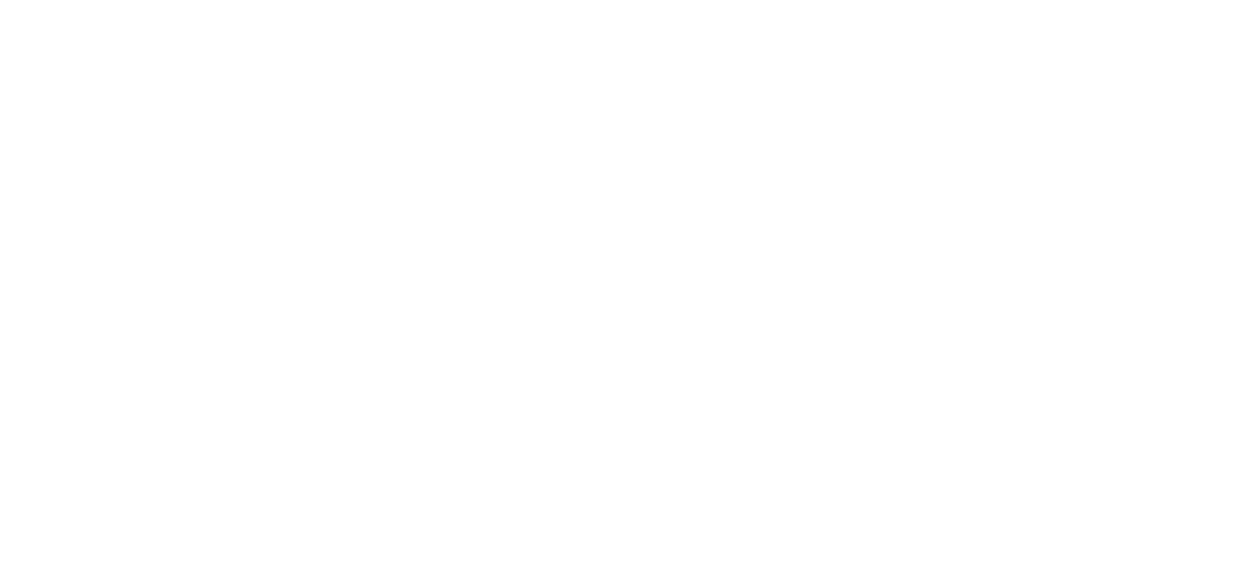
\includegraphics[scale=0.5]{images/image_binarisation_activity.pdf}
  \caption{An activity diagram to depict the design of the algorithm for the image segmentation.}
  \label{fig:activity_binarise}
\end{figure}

Figure \ref{activity_binarise} shows the overall activity of how the image processing will be intended to be implemented, after early design work showed binarisation was more complex. Further descriptions of specific implementation can be found in the implementation section.

This high-level activity diagram was the result of continuous design in the first few sprints. Initially a design was drawn up to just binarise the whole image, but due to implementation issues, this caused too much noise. Therefore, a new algorithm had to be established.

The blue-lined paper was one way to overcome that. Filtering the lines from a solid lined paper, would ensure less noise was on the image, creating a better binarised image. Overall, the activity diagram depicts the algorithm of taking a mobile phone photo, filtering the lines, binarising the image and extracting a tiff image. The tiff was selected as a design decision, as Tesseract input requires a tiff file.

This design initially considered blue to be important, but it was produced too much noise in the implementation. As a result, instead of trying to extract the lines, it was decided that the lines should be filtered and we should only extract the text. This was the final iteration of development on the binarisation script.

\section{Tesseract}
Early on in the sprints Tesseract was identified as the OCR tool of choice. Evaluations into the different tools available: [CITE - Case study] performs a case study using Tesseract as their OCR tool to analyse printed text in an image. Patel et al, also discuss the comparison against a proprietary OCR tool, Transym [CITE].

The results concluded by Patel et al is that Transym only yielded a 47\% accuracy on 20 images compared to 70\% accuracy using the Tesseract engine.

The first few iterations gave a concrete overview that the first three lines of the text would be parsed, forming the information for the meta-data. Appendix \ref{} shows the layout of the three lines.

\section{Entity-relation design}
Whilst creating the CRC cards, it allowed considerations to be made about the relations and how they are connected. Through each user-story analysed it was reflected upon if that would affect the entity-relation design.

\begin{figure}[h]
  \centering
  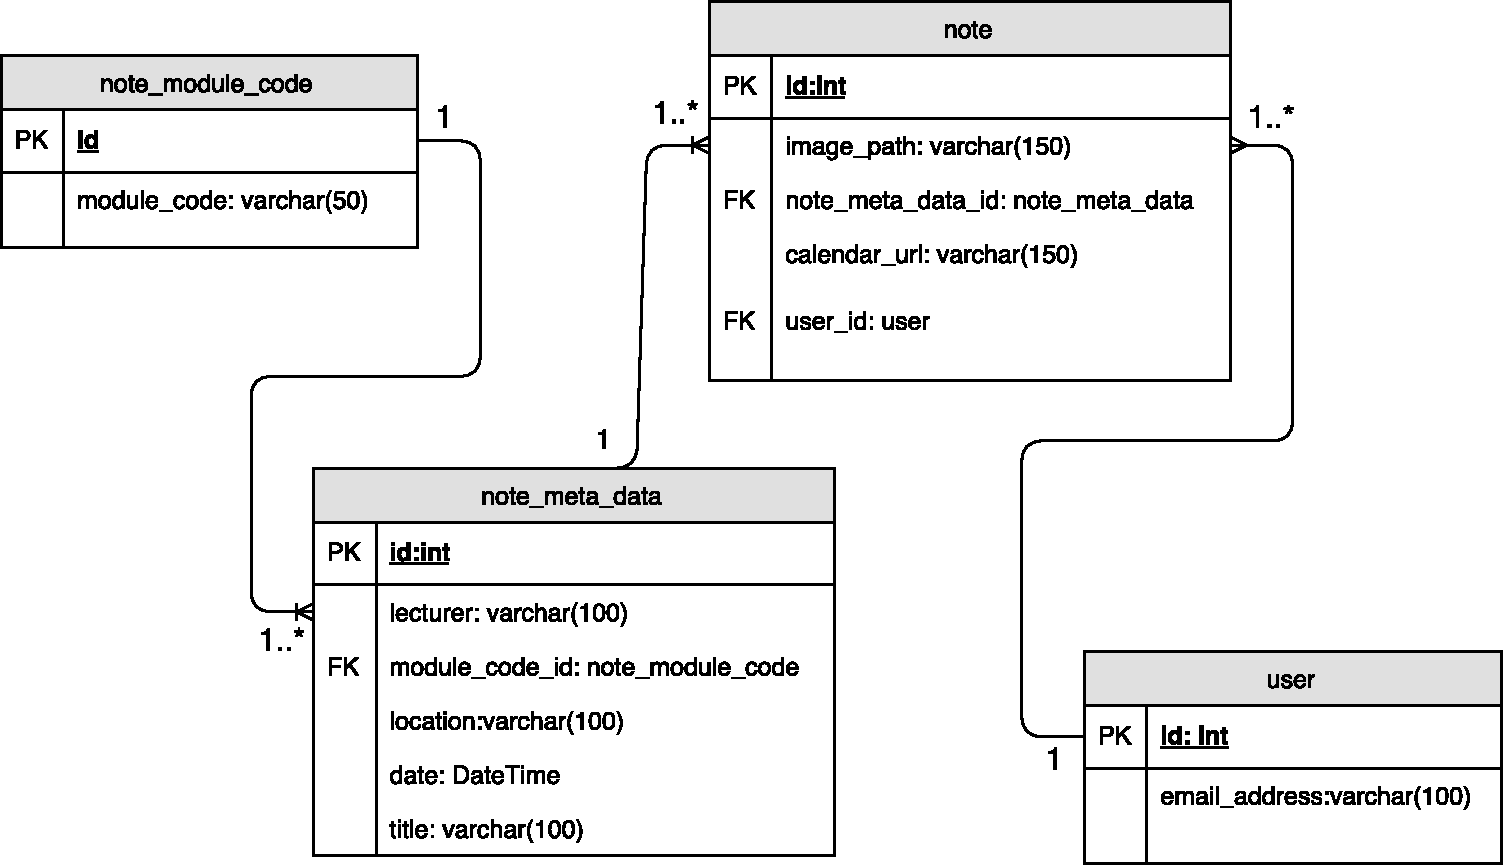
\includegraphics[scale=0.5]{images/database_diagram}
  \caption{The final result of the entity-relation diagram. After a series of iterations.}
  \label{fig:database}
\end{figure}

Figure \ref{fig:database}, shows the output from the result of continuous design on the database diagram through the iterations. The design per iteration matched that of the story. For example, although Meta-Data was known to be added into the system, this was not added until that story was brought into the sprint - instead just a Note relation was created.

\subsection{Justification of design}
Below is a justification of the designs through the iterations.
\subsubsection{Note}
During design persisting the note was one of the first entity-relation design decisions which was made. The attributes selected for the \texttt{Note} relation best justify what a note consists of. Firstly, the note contains an image link, which is a relative path to the image. This was persisted to ensure that it could be found easily. When the story for implementing user's was actioned, an additional field containing the user's id was added to the relation.

During the implementation of adding a URL to a calendar event, the calendar URL was persisted to the database of the associated note. The event ID could have be saved, but the URL was decided to stored so additional queries were not made to the external service. Furthermore, a note will only have one URL.

When implementing the note's meta-data, a relation was created and the foreign key was added to the note relation. This was created to ensure that a note must have associated meta-data.

\subsubsection{Note_meta_data}
The \texttt{note_meta_data} relation was created in its own relation to reduce data-redundancy, following the principle of normalisation in relational databases. The content could be duplicated for multiple notes, if a user tags the same meta-data to more than one note. As denoted from the relationships: a note will have a singular meta-data item, but the meta-data item could have many notes.

With attributes lecturer location and datetime - these were the initial design decisions made to be included in the meta-data. However, in a later iteration it was decided a title would be preferable; this was added to the relation. The date field is a date-time instead of a string due to integration with the calendar requires specific date-time strings, making it easier to parse.

Initially developed with the module code in this relation, in subsequent iterations the module code was extracted and a foreign key was used.

\subsubsection{Module code}
The module code was developed into its own relation to prevent data-redundancy. A user may enter multiple notes for the same module code - as a result the database would only need to include one reference of that module code. The relationship between the meta data and the module code is explicit: the meta data must contain one module code but the module code can have more than one meta-data item.

\subsubsection{User}
This was not added to the application until around sprint 5. Details regarding oAuth can be found in \ref{}. However, the user will have an email address and that would be stored. It is in its own relation from a logic perspective: every time a user signs up to the system they are not creating a note instantly, therefore a relation was created to separate this logic. The foreign key was added to a note, so that a note can only have one user - and a user can have multiple notes.


\noindent
Overall, a succinct collection of relations have been developed which aim to solve the issues of the data-redundancy, by providing solid rationale for the resulting design.


\section{Sprints}

\section{User interface}
With the web application being a core part a series of user interfaces (UI) was collated at the start of each breakdown of the story - if there was a significant change in the UI.

The user interface had make the web application feel like an application, rather than a traditional website. This was identified from the background analysis where many systems felt like an application. The colour scheme was aiming to be simplistic, using the Google colour style guide. An alternative of bootstrap was considered, instead of designing bespoke CSS. Although it has a built-in responsive theme, due to the over-kill of the additional files a simpler approach was adopted.

\begin{figure}
  \centering
  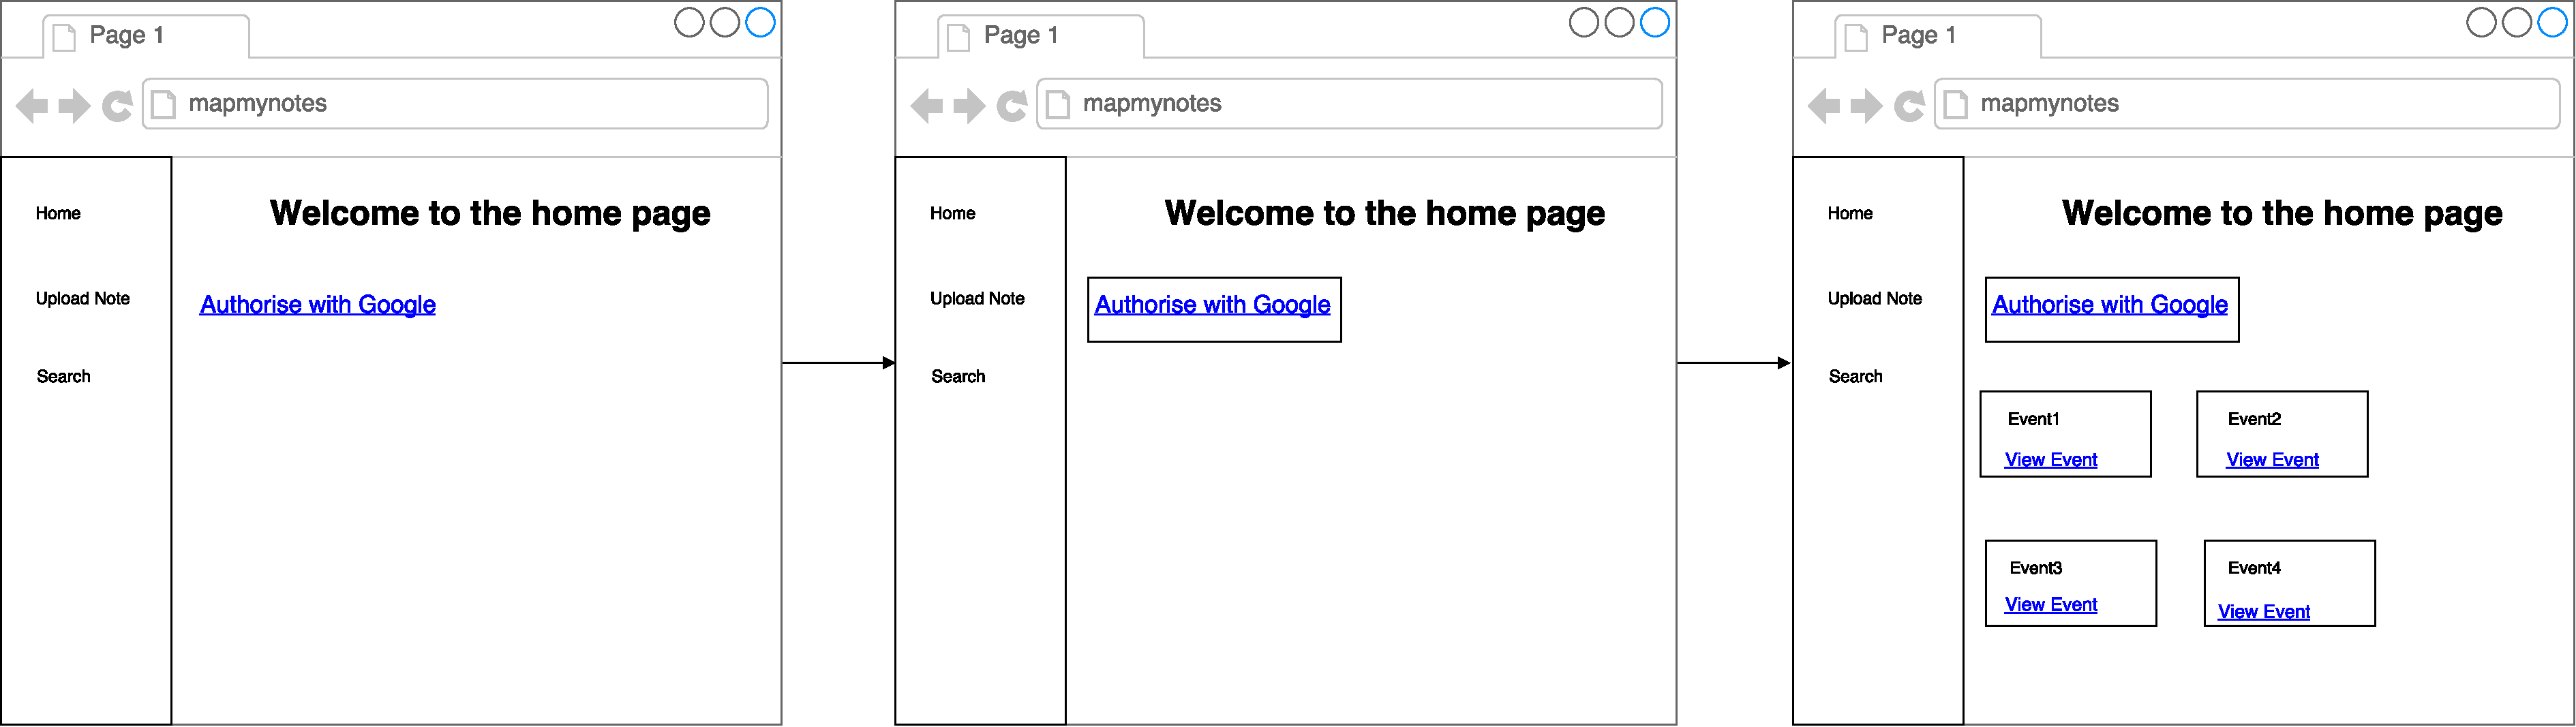
\includegraphics{images/homepage_wiremock.pdf}
  \label{fig:homepage_wiremock}
  \caption{From left to right, the homepage wiremock through the different iterations and the change of requirements}
\end{figure}

Figure \ref{fig:homepage_wiremock} shows the exploratory wiremock design completed prior to the UI interface. From the early iterations it was just an authorise button, then as a requirement was added to show the user events from the last seven days it was mocked up to reflect this.


Further mockups available in Appendix \ref{}.


\section{Implementation tools}
The following sections discuss the implementation tools and their purpose within the application.
\subsection{Programming language}
The programming language would not change per sprint or over an iterative process - as a result this was identified in sprint 0, where additional spike work was completed.

As a web application was being developed investigatory work was completed into the analysis of suitable server-side languages. Typically traditional server-side applications language are: PHP, Ruby, Python, C\#, Java and JavaScript, which has increased in popularity \cite{citeulike:14018462}.

Decomposing the analysis in the early sprints determined that OpenCV would be utilised on the project. OpenCV's source code is written in C++, however Python and Java bindings are available. Additional research was conducted to see if a reliable wrapper for either PHP or Ruby was available, and after a lot of investigation it was concluded there was not.

C++ is not considered a standard web application development language removing it as a viable option for the web application. Java applications are predominately large commercial applications, using a range of enterprise software - often renowned for their performance abilities \cite{citeulike:14019744}. This approach felt too cumbersome for a proposed light-weight application.

By being constrained by design decisions to use OpenCV and a reluctance to use Java, then Python was selected as the most suitable language. Python offers a lightweight and an easy to learn syntax that produces readable code, allowing a object-oriented paradigm to be followed. Additionally, its support for OpenCV is sufficient for the application.

\subsection{Framework}
As Python was being used as the language of choice, this narrowed down the frameworks available. Frameworks are useful for handling more complex features like routing and session handling - leaving the developer to focus on more domain specific issues.   Exploratory work was completed in the early sprints to find a suitable tool. The frameworks Django \cite{citeulike:14019784}, Flask \cite{citeulike:13160396} and Bottle \cite{citeulike:14019792} were evaluated.

Some frameworks constrain the developer's to specific implementations through abstracted classes whereas some offer more flexibility. Whilst evaluating Django, a full framework, it was concluded that such a large framework was excessive for this application and rejected as a choice for the framework.

Flask and Bottle are classified as ``micro-frameworks'', offering a lightweight structure, allowing developers to have more control on the structure. On face value, Flask and Bottle appear to be very similar; they are both lightweight with a similar syntax. After evaluation both frameworks it was concluded that Flask has a larger support community compared to Bottle - along with more reliable documentation.

As a result, Flask was chosen as the framework which will be used throughout the application. Spike work was completed into evaluating Flask's viability for the application and was decided to be a good choice.

\subsection{Continuous integration tools}
Continuous Integration (CI) is normally used in development teams to ensure that all code is checked into the repository. As it was changed for a single person project, so did the point of using it; it was used to ensure every commit passed all tests when pushing to the repository.

After identifying CI would be used in the analysis stage, an appropriate tool would have to be chosen. Jenkins was an initial choice; it is a standalone Java application which a repository can be synced to.

Travis CI, is a CI tool in the cloud which can be synced to a GitHub repository. Tests can be run during every commit of the application and details regarding if it errors, passes or fails is available.

A key design decision was to be able to check the build process quickly. With Travis it has a web interface clearly showing the output. Jenkins would require additional set up of specific build scripts for every branch in the application. Travis would be easier to set up and would easily integrate with the application.

\subsection{Version control}
Version control was used on the project to ensure that code was under specific versions. The project was created on a private Git repository on GitHub. Git was chosen for its familiarity and GitHub is a well known place for handling Git based solutions; Travis CI integrated well with GitHub.

It is worth making a mention on the Git flow which was used. As each story was implemented a branch would be created in the form of: \texttt{feature/<summary_of_story>}, such as \texttt{feature/logout}. Branches were created from the development branch. All code was pushed to its own separate branches, and only when Travis CI passed a pull request was created on GitHub.  Once Travis had successfully passed all the pull request tests, and it was safe to merge then the branches were merges into development.

\subsection{Development environment}
The text-editor, Atom, was used for the majority of the project. It was a lightweight tool which accommodated for Python syntax. However later in the project, when refactoring became more cumbersome due to the increase in code base - PyCharm community edition was used as it offered better refactoring functionality.
